\chapter{Dema funkcjonalności}
Poza samymi testami zaimplementowane zostało także kilka programów typu demo, przedstawiających poszczególne funkcjonalności modułu.

\section{Moduł rdzeniowy}
Ze względu na fakt, iż założenie modularności było jednym z najważniejszych aspektów projektowania projektu, testy i dema zostały podzielone na segmenty, pokazujące różne formy użycia gotowego API modułu. Początkowe testy skupią się na najważniejszym komponencie - warstwie rdzeniowej.

\subsection{Minimalne okno i konfiguracja Direct3D 11}
Pierwszym demem, podstawą prawie każdego projektu opartego o API Direct3D, a jednocześnie testem działania modułu rdzeniowego jest program, którego celem jest utworzenie minimalnej pętli Clear(), Present(), czego efektem będzie wyczyszczony stałym kolorem obraz na nowo otwartym oknie, a także obsługa interakcji użytkownika z tymże oknem.

Utworzenie takiego programu jest banalnie proste przy pomocy API utworzonego modułu i z wyłączeniem komentarzy wymaga od aplikacji klienckiej jedynie 10 linijek prostego kodu, przedstawionego na listingu \ref{lst:demo:core:minimalWindow}. Jako porównania użyć można wzorcowego projektu zawartego w programie Visual Studio, który realizuje taką samą funkcję, ale wykonuje to znacznie bardziej złożonym kodem o objętości około 1000 linijek.

\vfill

\begin{lstlisting}[caption={Pełny kod programu wykorzystującego API modułu do utworzenia minimalnego okna.}, label={lst:demo:core:minimalWindow}]
	#include <URM/Core/D3DCore.h>
	
	int WinMain(HINSTANCE hInstance, HINSTANCE, LPSTR, int nCmdShow) {
		// Utworzenie struktury D3DCore z przekazaniem parametrów kreacji. 
		URM::Core::D3DCore core(
			URM::Core::WindowCreationParams(
				800,            // Szerokość okna
				600,            // Wysokość okna
				"EmptyWindow",  // Tytuł okna
				hInstance       // Uchwyt do instancji WinAPI
			)
		);
	    
		// Główna pętla programu działająca do momentu zamknięcia okna.
		while(!core.GetWindow().IsDestroyed()) {
			// Obsługa zdarzeń okna.
			core.GetWindow().PollEvents();

			// Czyszczenie zawartości okna zdefiniowanym kolorem.
			core.ClearFramebuffer(DirectX::SimpleMath::Color(0.3, 0.5, 1.0));

			// Prezentowanie wygenerowanej klatki obrazu na ekran.
			core.Present(0);
		}
	}
\end{lstlisting}

\subsection{Wczytanie i wyświetlenie prostego modelu}
Podstawowym i najważniejszym z zadań program renderującego jest rysowanie modeli w przestrzeni. Aby pokazać możliwości związane z tym tematem, kolejnym przykładem została aplikacja rozbudowująca przykład poprzedni o trójwymiarowy sześcian wyświetlany w utworzonym oknie. Moduł rdzeniowy oddaje do dyspozycji pełną kontrolę nad całym procesem aplikacji klienta, ułatwiając przy tym pracę nad niskopoziomowym API Direct3D, co pozwoliło na znaczącą redukcję złożoności tak powstałego programu do mniej niż 170 linijek kodu, a czego efekty zostały przedstawione na rys. \ref{demo_core_cube}. Przedstawiają one omawiany model z użytym niestandardowym programem cieniującym, wyświetlającym wartość wektora normalnego powierzchni jako jej kolor. 

\begin{figure}[h!]
	\centering
	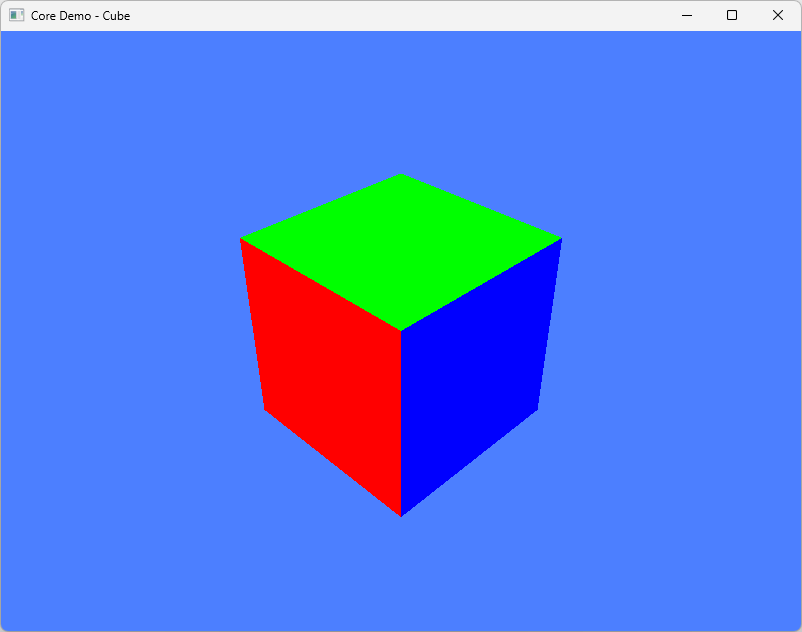
\includegraphics[width=\textwidth]{images/demo_core_cube.png}
	\caption{Kolorowy model sześcianu narysowany przy pomocy API modułu rdzeniowego.}
	\label{demo_core_cube}
\end{figure}

\section{Moduł silnika}
W poniższej sekcji przedstawione zostały dema wykorzystujące API warstwy silnika, mające na celu ukazanie możliwości oraz elastyczności opisywanego modułu.

\subsection{Wczytanie i wyświetlenie prostego modelu - c.d.}
Mimo względnie niskiej objętości kodu potrzebnego do utworzenia przykładowych aplikacji przy pomocy modułu rdzeniowego, jest on już na tym etapie wyraźnie złożony. Do działania wymagane jest kontrolowanie stanu modułu rdzeniowego, stanu rasteryzera, viewport'u, shader'ów, InputLayout, buforów stałych i zmiennych, a także wczytanych modeli. Moduł silnika przejmuje na siebie obowiązki związane z zarządzaniem tymi zasobami, udostępniając przy tym przejrzyste API, bez ograniczania możliwości hybrydowego użycia z niższymi warstwami. 

Rekreacja wcześniej opisanego dema przy pomocy nowego API silnika było wyjątkowo proste i zmniejszyło objętość aplikacji klienta do około 30 linijek kodu. Kod opisywanego dema, będący jednocześnie przykładem użycia interfejsu modułu silnika został przedstawiony na listingu \ref{lst:demo:engine:cube}. Poza wyraźnym uproszczeniem pracy z takim systemem, konwersja na API silnika umożliwia też łatwe rozszerzenie funkcjonalności o dodatkowe modele, różne materiały i shader'y, czy oświetlenie. Pokazane to zostało na rys. \ref{demo_engine_cube}, gdzie do widocznej już wcześniej kolorowej kostki dodane zostały dwa bliźniacze do niej sześciany, wykorzystujące zupełnie inne materiały i programy cieniujące.

\begin{figure}[h!]
	\centering
	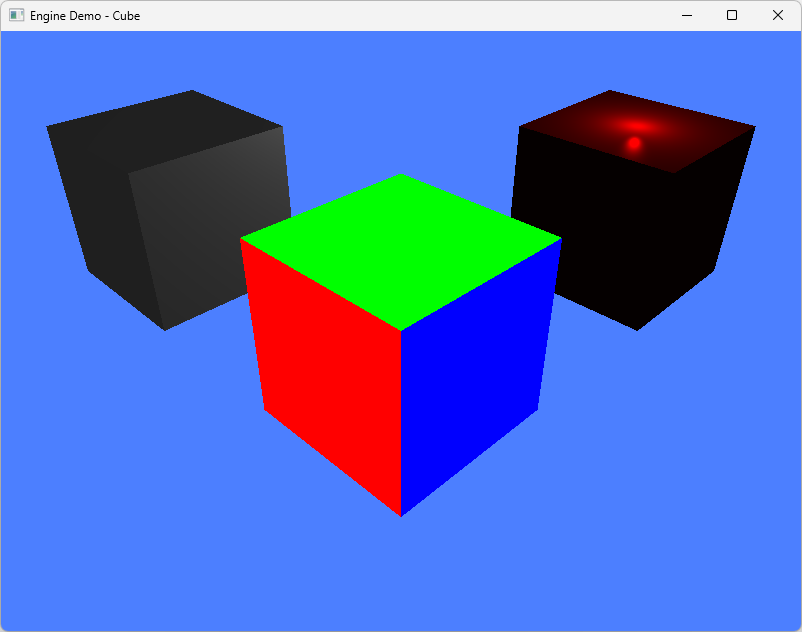
\includegraphics[width=\textwidth]{images/demo_engine_cube.png}
	\caption{Rozszerzone demo sześcianu utworzone przy pomocy interfejsu modułu silnika.}
	\label{demo_engine_cube}
\end{figure}

\vfill

\begin{lstlisting}[caption={Pełny kod programu wykorzystującego API silnika do wyświetlenia trzech sześcianów o różnych materiałach.}, label={lst:demo:engine:cube}]
#include <URM/Engine/Engine.h>
#include <URM/Engine/CameraObject.h>
#include <URM/Engine/ModelObject.h>
#include <URM/Core/StandardMaterials.h>

using namespace URM::Core;
using namespace URM::Engine;

// Definicja nowego typu materiału o niestandardowym progarmie cieniującym
struct NormalColorMaterial : public Material {
	const wchar_t* GetShaderFilePath() const override { 
		return L"NormalColorPixelShader.cso";
	}
};
	
int WinMain(HINSTANCE hInstance, HINSTANCE, LPSTR, int nCmdShow) {
	// Utworzenie instancji silnika z parametrami okna
	Engine engine(WindowCreationParams(800, 600, "Engine Demo - Cube", hInstance));
	// Ustawienie koloru tła
	engine.renderParameters.clearColor = Color(0.3f, 0.5f, 1.0f);
	
	// Utworzenie głównej kamery wraz z pozycją i kierunkiem
	auto camera = std::make_shared<CameraObject>(45.0f);
	camera->GetTransform().SetPosition({ 4.0f, 4.0f, 4.0f });
	camera->GetTransform().LookAt({ 0.0f, 0.0f, 0.0f });
	// Ustawienie kamery jako głównej kamery w scenie
	engine.GetScene().SetMainCamera(camera);
	engine.GetScene().GetRoot().lock()->AddChild(camera);
	
	// Dodanie punktu światła do sceny
	engine.GetScene().GetRoot().lock()->AddChild(new LightObject());
	
	// Utworzenie obiektu z niestandardowym materiałem / shader'em
	auto material = std::shared_ptr<NormalColorMaterial>(new NormalColorMaterial());
	auto cube = engine.GetScene().GetRoot().lock()->AddChild(
		new ModelObject("cube.glb", material)
	);
	
	// Uruchomienie pętli silnika
	engine.RunLoop();
}
\end{lstlisting}

\subsection{Manualna kontrola procesu rysowania}
Moduł silnika poza automatycznym systemem zarządzania przepływem działania programu, umożliwia także jego ręczną kontrolę z poziomu aplikacji klienta. Przedstawiona w tej sekcji aplikacja jest przykładem takiego podejścia. Zdarzeniem warunkowym może być dowolny sygnał, ale w przypadku dema proces rysowania odbywa się tylko jeśli użytkownik wciska przycisk "R" na klawiaturze. Kod reprezentujący sposób takiej pracy został przedstawiony na listingu \ref{lst:demo:engine:manualDrawingLoop}.

\begin{lstlisting}[caption={Kod przykładowego programu manualnej kontroli przepływu działania programu w module silnika.}, label={lst:demo:engine:manualDrawingLoop}]
	// Utworzenie instancji silnika z parametrami okna
	Engine engine(...);
	
	// Przygotowanie sceny - dodanie modelu, kamery, oświetlenia
	...
	
	// Pobranie uchwytu do klawiatury
	auto keyboard = engine.GetScene().GetCore().GetKeyboard();
	
	// Ręczna pętla rysowania
	float rotation = 0.0f;
	while (!engine.ShouldClose()) {
		// Aktualizacja zdarzeń - dzięki temu okno pozostaje reponsywne
		engine.Update();
		
		// Rysowanie sceny tylko jeśli klawisz 'R' jest wciśnięty
		if(keyboard.lock()->GetState().IsKeyDown(DirectX::Keyboard::R)) {
			rotation += engine.GetTimer().GetDeltaTime() * 90.0f;
			model->GetTransform().SetLocalRotation({ 0.0f, rotation, 0.0f });
			
			// Ręczne czyszczenie, rysowanie i prezentacja
			engine.Clear(Color(0.3f, 0.5f, 1.0f));
			engine.Draw(engine.renderParameters);
			engine.Present(0);
		}
	}
\end{lstlisting}

\subsection{Sponza}
Stworzona pierwotnie przez Marko Dabrovic'a, następnie ulepszona przez niemiecką firmę Crytek \cite{github:Khronos:Sponza}, a w 2022 roku ponownie usprawniona przez amerykańskiego giganta Intel \cite{Intel:GPUResearch:Sponza} reprezentacja rzeczywistego atrium pałacu Sponza, znajdującego się w Chorwackiej miejscowości Dubrovnik stała się jednym z najpopularniejszych modeli służących do testowania i porównywania programów grafiki 3D, a w szczególności modułów odpowiedzialnych za oświetlenie globalne. W ramach tej sekcji przedstawiona została najprostsza wersja od firmy Intel w dwóch wersjach - uproszczonej oraz PBR. W obu manualnie dobrane zostało oświetlenie oraz kolor nieba celem utworzenia kompozycji reprezentującej zbliżone do realnego zastosowanie modułu. W poniższej tabeli przedstawiona została także zmierzona wydajność renderowania, a wygenerowane zrzuty ekranu na rys. \ref{test_sponza_1}, \ref{test_sponza_2} i \ref{test_sponza_3}.

\begin{center}
	\begin{tabular}{ |l r r r|}
		\hline
		\textbf{Układ graficzny} & \textbf{FPS - uproszczony} & \textbf{FPS - PBR} & \textbf{Wydajność PBR} \\
		\hline
		NVIDIA 4060 & \textbf{955} & \textbf{718} & \textbf{75.18\%} \\
		Radeon 780M & \textbf{380} & \textbf{287} & \textbf{75.53\%} \\
		Procent wydajności & \textbf{39.79\%} & \textbf{39.79\%} & - \\
		\hline
	\end{tabular}
\end{center}

	
\begin{figure}[h!]
	\begin{subfigure}{.5\textwidth}
		\centering
		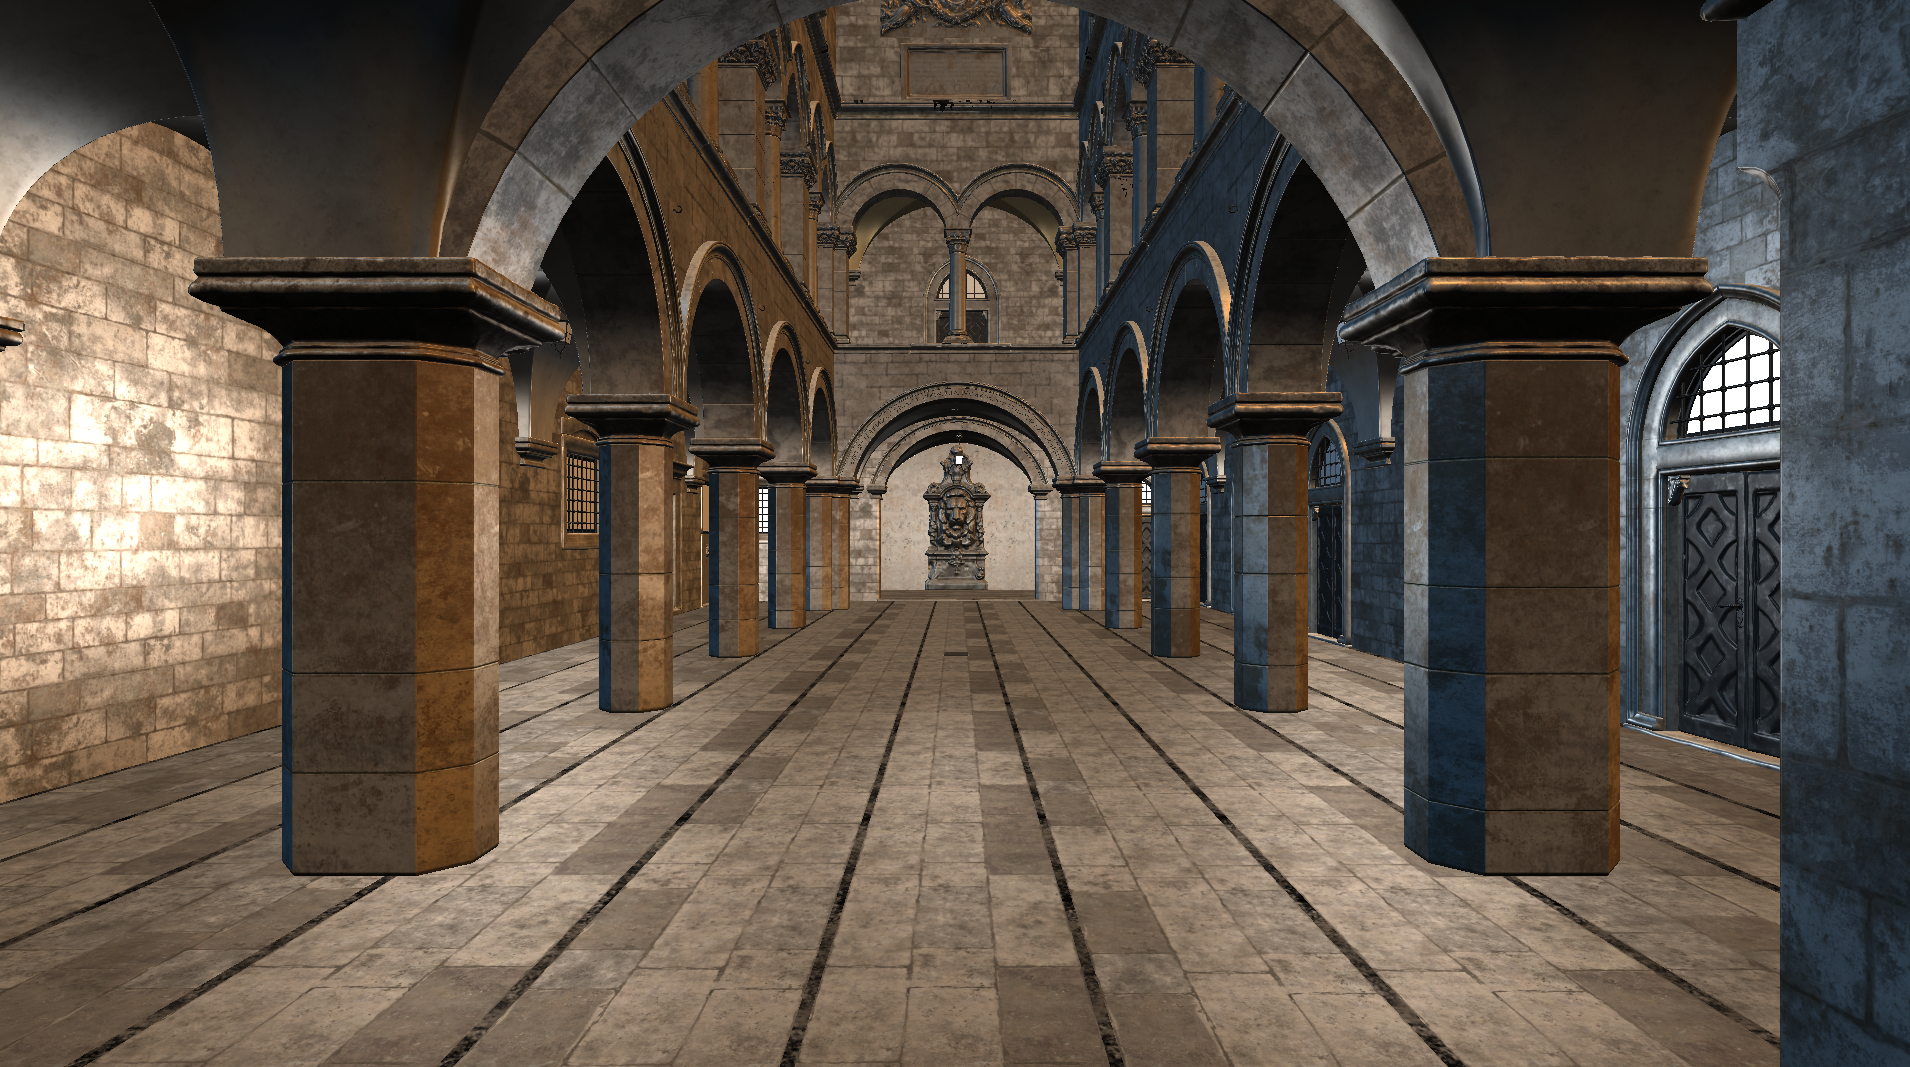
\includegraphics[width=\textwidth]{images/demo_sponza_1.png}
		\caption{Widok uproszczony.}
	\end{subfigure}
	\begin{subfigure}{.5\textwidth}
		\centering
		\includegraphics[width=\textwidth]{images/demo_sponza_1_pbr.png}
		\caption{Tryb PBR.}
	\end{subfigure}
	\caption{Hala atrium Sponza wygenerowana przez moduł.}
	\label{test_sponza_1}
\end{figure}

\begin{figure}[h!]
	\begin{subfigure}{.5\textwidth}
		\centering
		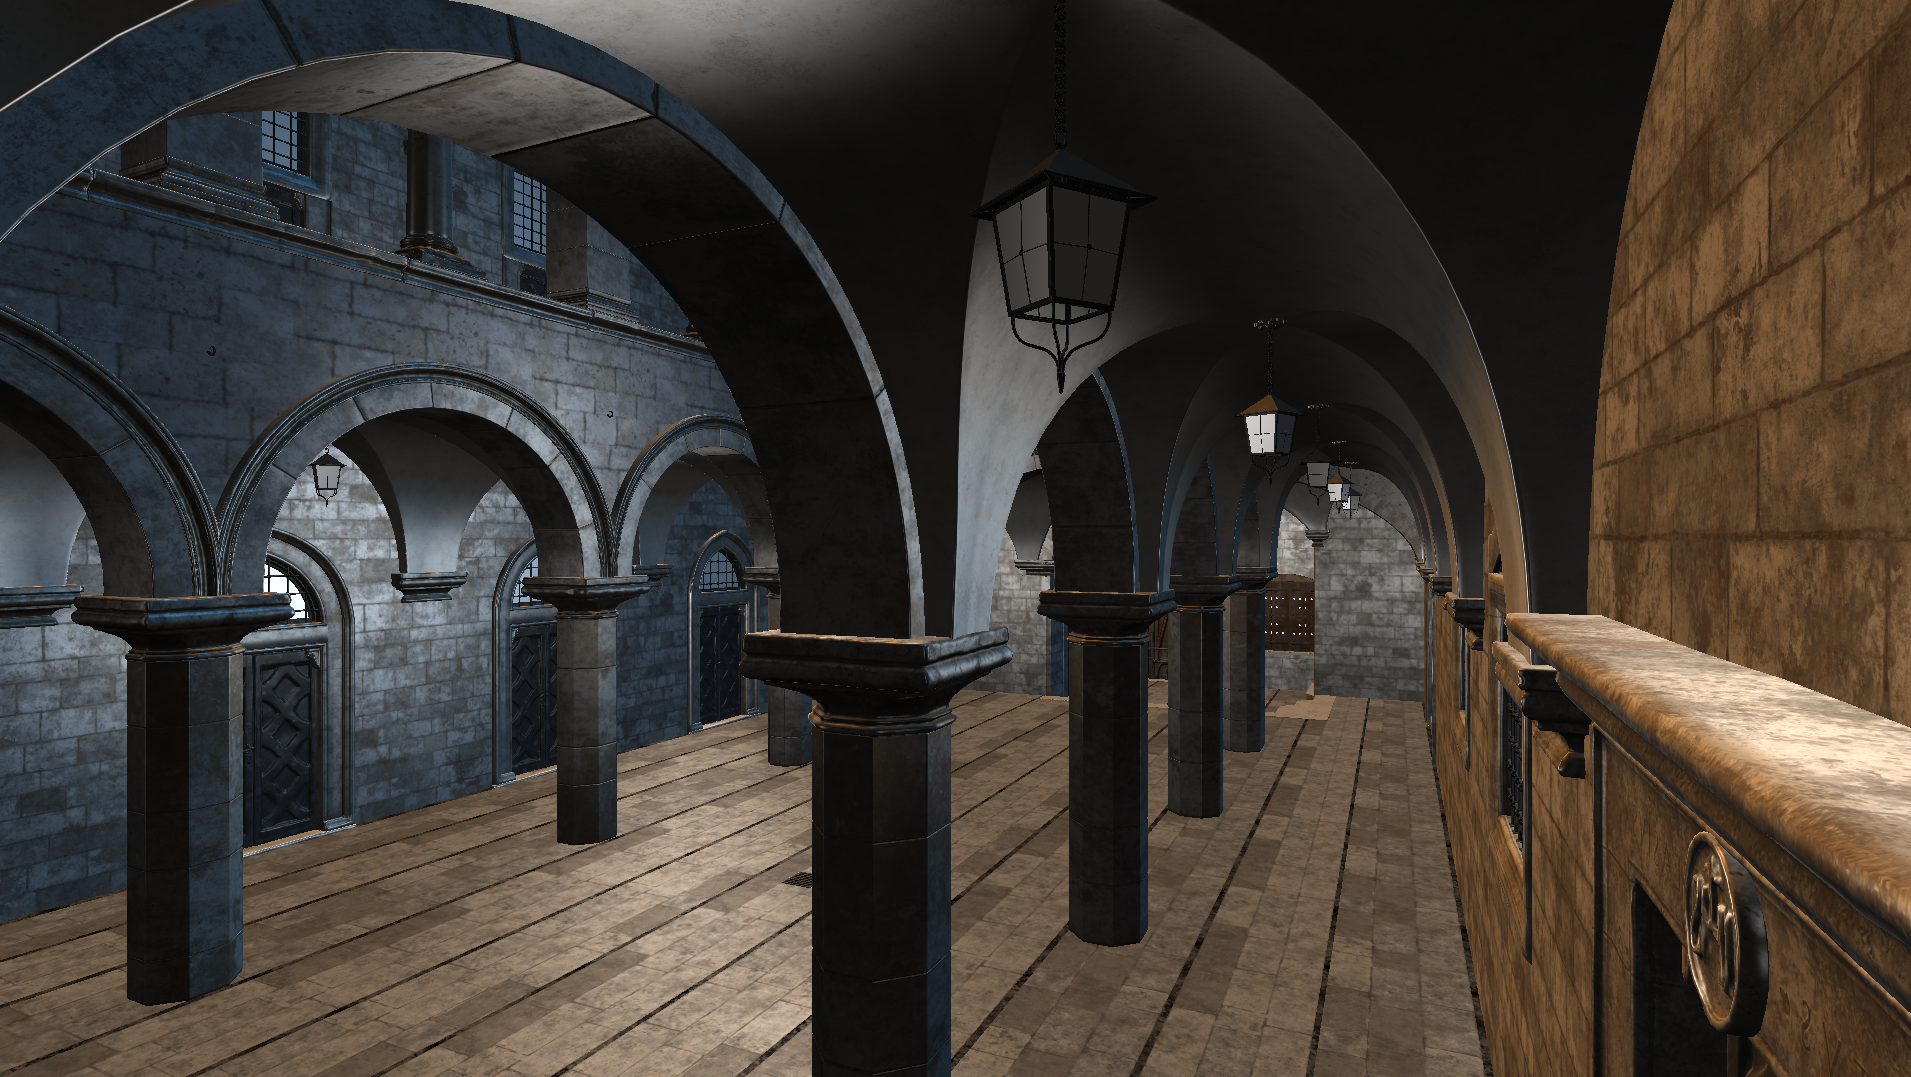
\includegraphics[width=\textwidth]{images/demo_sponza_2.png}
		\caption{Tryb klasyczny.}
	\end{subfigure}
	\begin{subfigure}{.5\textwidth}
		\centering
		\includegraphics[width=\textwidth]{images/demo_sponza_2_pbr.png}
		\caption{Widok PBR.}
	\end{subfigure}
	\caption{Zakrzywione stropy w korytarzach Sponza.}
	\label{test_sponza_2}
\end{figure}

\begin{figure}[h!]
	\begin{subfigure}{.5\textwidth}
		\centering
		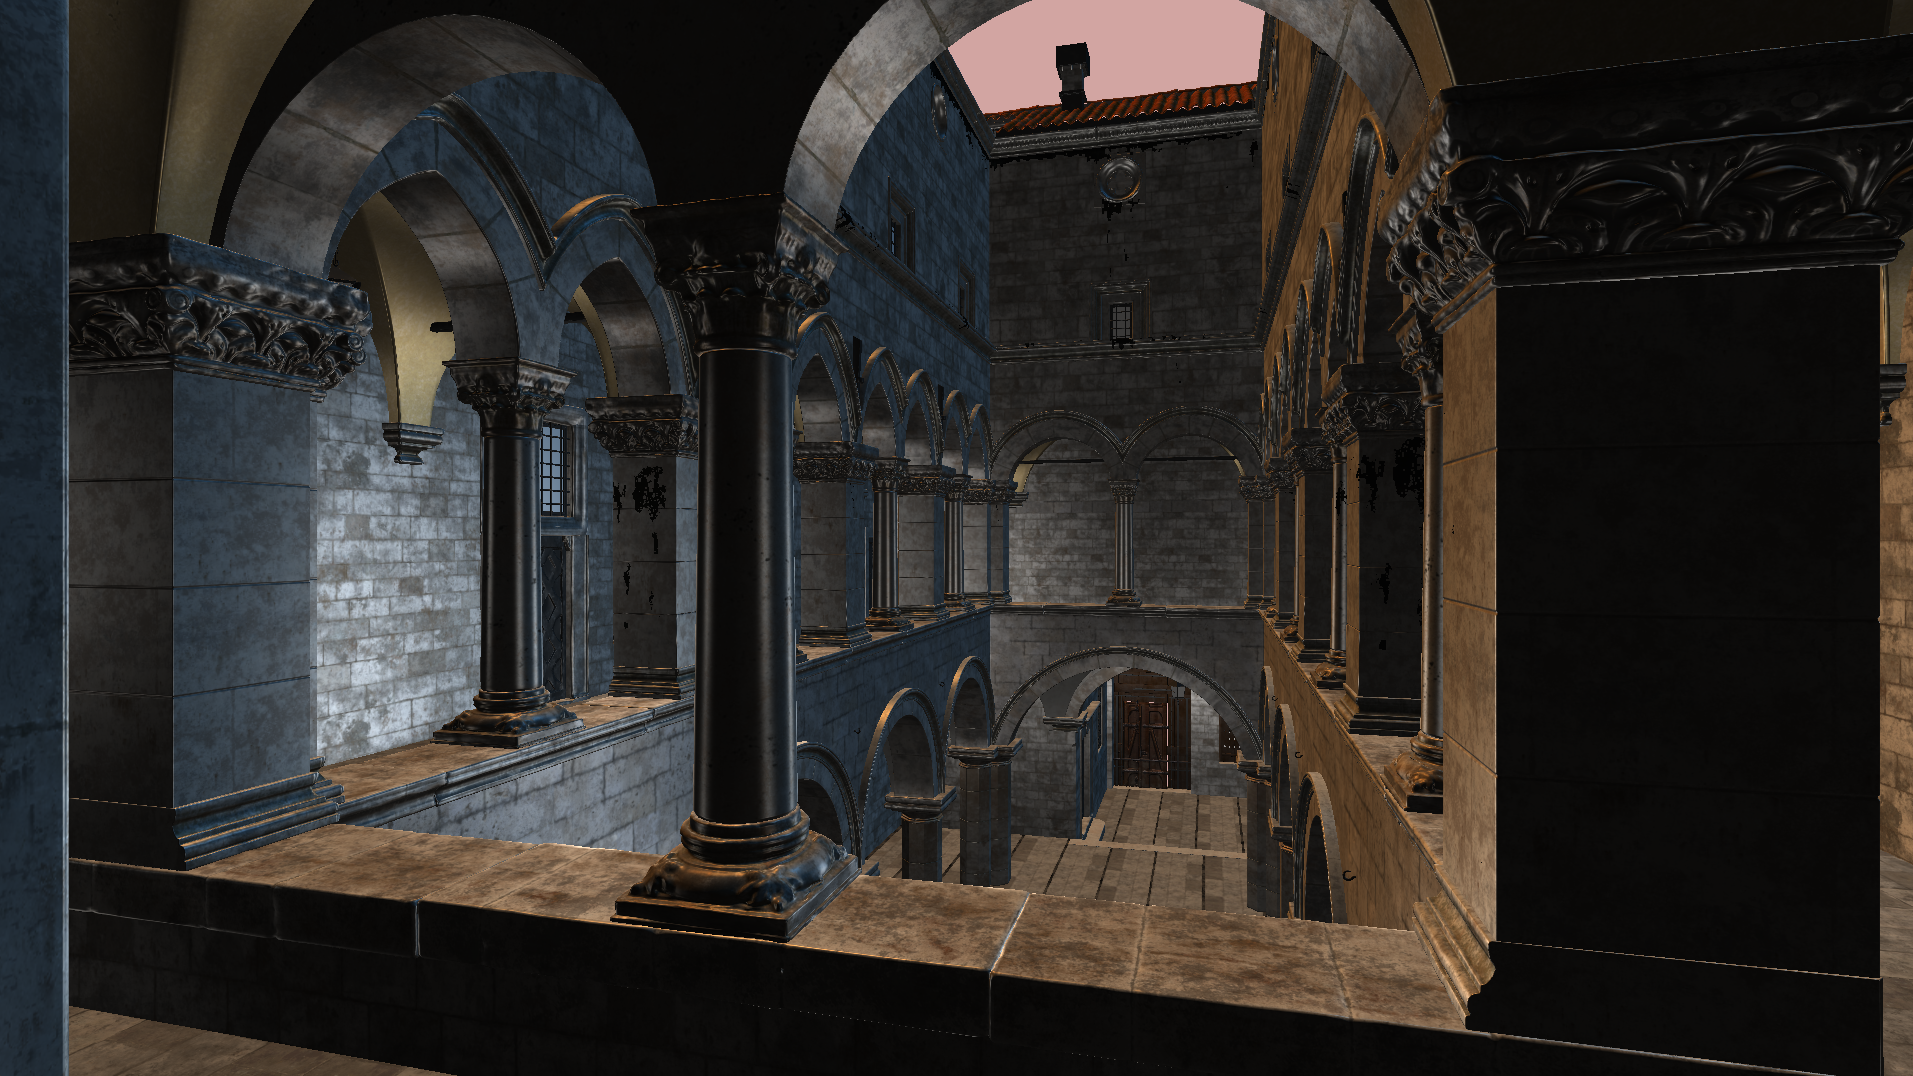
\includegraphics[width=\textwidth]{images/demo_sponza_4.png}
		\caption{Shader uproszczony.}
	\end{subfigure}
	\begin{subfigure}{.5\textwidth}
		\centering
		\includegraphics[width=\textwidth]{images/demo_sponza_4_pbr.png}
		\caption{Wersja oparta o Physically Based Rendering.}
	\end{subfigure}
	\caption{Widok z piętra pałacu.}
	\label{test_sponza_3}
\end{figure}

\vfill
\clearpage

\subsection{Demo detali - Roman Marble Plinth}
Opisywany już w rozdziale testów model \textit{Roman Marble Ornate Plinth} z pakietu Quixel Megascans został głównym obiektem tej sekcji, ze względu na dużą ilość detali geometrii i tekstur. Przedstawiony w dwóch wersjach na rys. \ref{test_highpoly} model charakteryzuje się wysokim narzutem wydajnościowym przy rysowaniu, co dało wyraźny znak przy określaniu wydajności dema, czego szczegóły zostały przedstawione w poniższej tabeli.

\begin{center}
	\begin{tabular}{ |l r r r|}
		\hline
		\textbf{Układ graficzny} & \textbf{FPS - uproszczony} & \textbf{FPS - PBR} & \textbf{Wydajność PBR} \\
		\hline
		NVIDIA 4060 & \textbf{360} & \textbf{445} & \textbf{123.61\%} \\
		Radeon 780M & \textbf{84} & \textbf{84} & \textbf{100.00\%} \\
		Procent wydajności & \textbf{23.33\%} & \textbf{18.88\%} & - \\
		\hline
	\end{tabular}
\end{center}

\begin{figure}[h!]
	\begin{subfigure}{.5\textwidth}
		\centering
		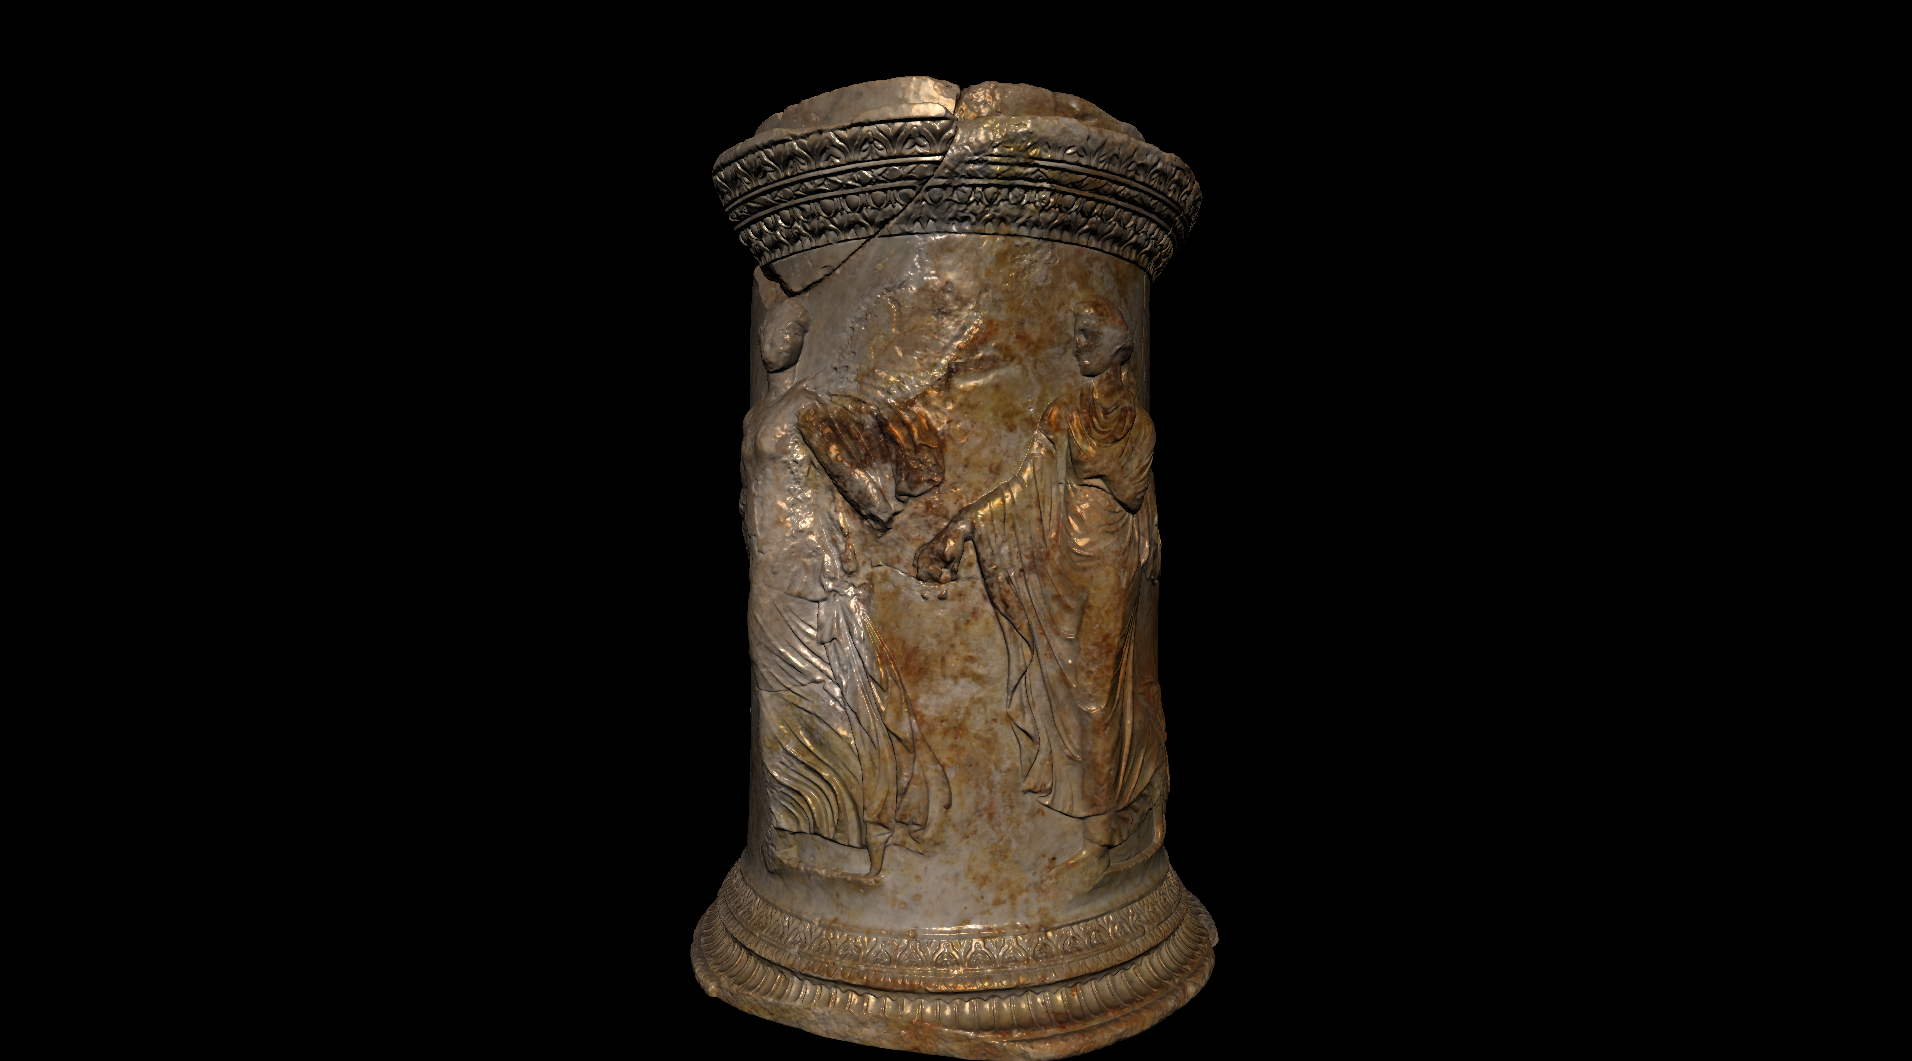
\includegraphics[width=\textwidth]{images/demo_highPoly.png}
		\caption{Wersja uproszczona.}
	\end{subfigure}
	\begin{subfigure}{.5\textwidth}
		\centering
		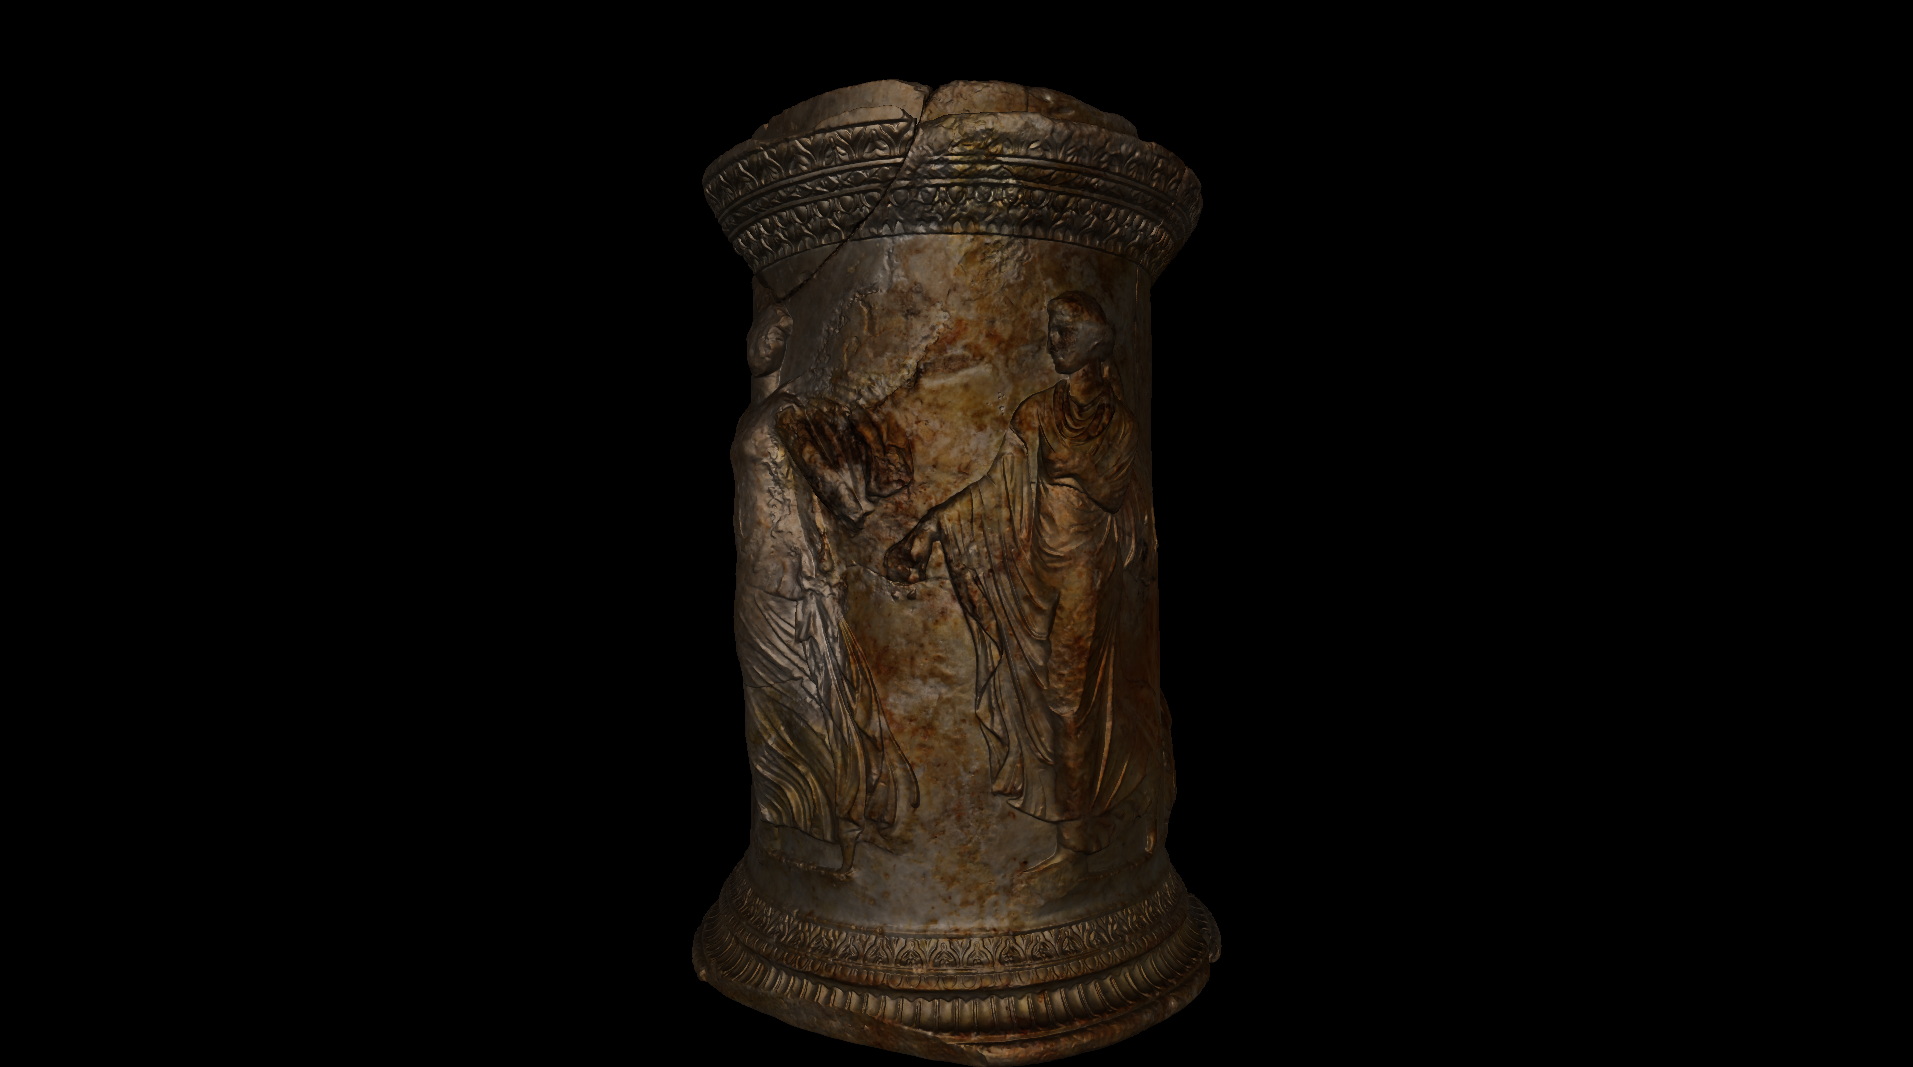
\includegraphics[width=\textwidth]{images/demo_highPoly_PBR.png}
		\caption{Tryb PBR.}
	\end{subfigure}
	\caption{Model cokołu w dwóch trybach działania modułu.}
	\label{test_highpoly}
\end{figure}

\subsection{Materiały}
Ostatnim demo przedstawiającym główne funkcjonalności modułu jest pokazanie możliwości zaimplementowanego systemu materiałów. Scena testu, pokazana na rys. \ref{demo_materials} składa się z 3 głównych części.
 
Głównym, środkowym elementem jest zbiór modeli kul o różnych parametrach materiałów. Elementy czerwone mają przypisany materiał typu PBR, a ich umieszczenie pokazuje różnice między jego parametrami. W osi pionowej od góry do dołu rośnie wartość chropowatości powierzchni - \textit{roughness}, a w poziomej od lewej do prawej parametr metaliczności. Kule zielone rysowane są przy pomocy uproszczonego materiału, a kolejne instancje zwiększają konfigurację chropowatości od lewej do prawej. 

Pozostałe segmenty przyjmują postać wydłużonych w pionie sześcianów, pokazujących bezproblemową możliwość doimplementowania dodatkowych materiałów. Wykorzystują one nowy materiał i przypisany do niego shader, niebędący częścią oryginalnego modułu, zwracający kolor odpowiadający pozycji na ekranie. Jego dwie instancje różnią się włączeniem i wyłączeniem kalkulacji oświetlenia, odpowiednio dla lewej i prawej wersji. 

Wygenerowana scena przedstawiona została na rys. \ref{demo_materials}.

\begin{figure}[h!]
	\centering
	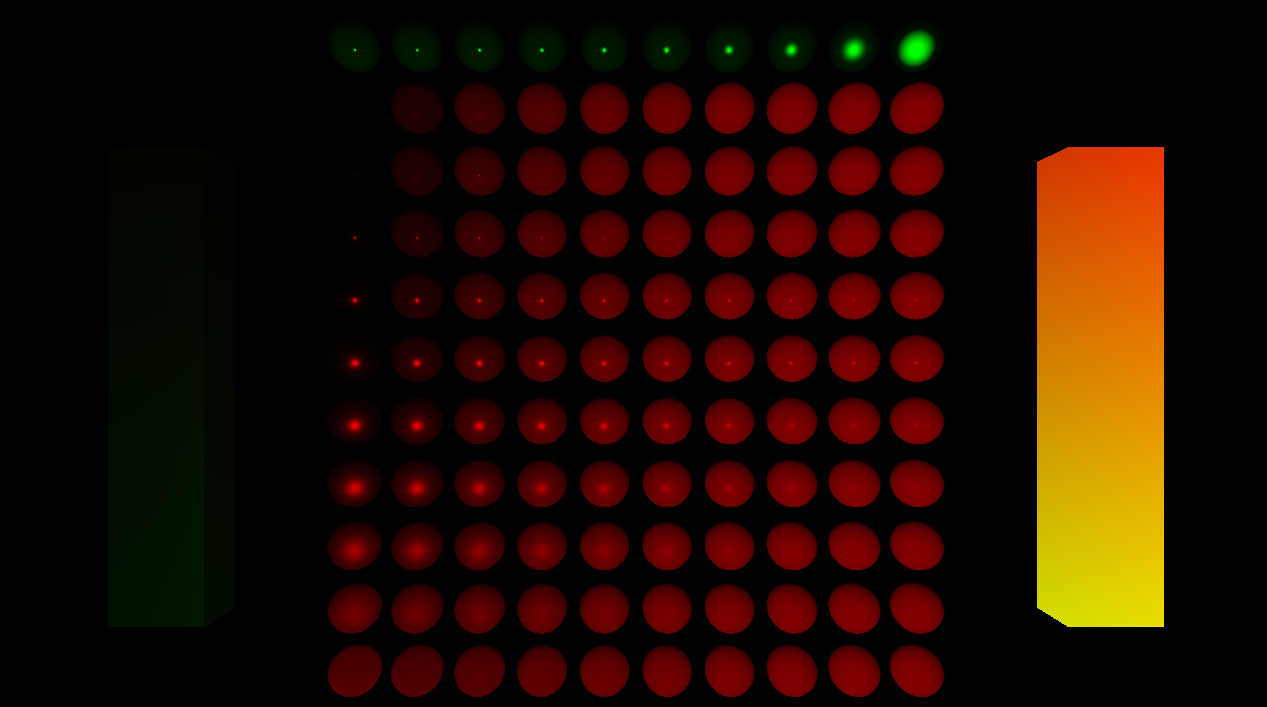
\includegraphics[width=\textwidth]{images/demo_materials.png}
	\caption{Zrzut ekranu przedstawiający obiekty o różnych materiałach i programach cieniujących.}
	\label{demo_materials}
\end{figure}